\documentclass[conference]{IEEEtran}
\IEEEoverridecommandlockouts
\usepackage[T1]{fontenc}
\usepackage{cite}
\usepackage{amsmath,amssymb,amsfonts}
\usepackage{algorithmic}
\usepackage{graphicx}
\usepackage{textcomp}
\usepackage{xcolor}
\usepackage{booktabs}
\usepackage{hyperref}
\usepackage{subcaption}
\usepackage[table]{colortbl}

\graphicspath{{figures/}}

\setlength{\textfloatsep}{8pt plus 2pt minus 2pt}
\setlength{\floatsep}{6pt plus 2pt minus 2pt}
\setlength{\intextsep}{6pt plus 2pt minus 2pt}
\setlength{\dbltextfloatsep}{8pt plus 2pt minus 2pt}
\setlength{\dblfloatsep}{6pt plus 2pt minus 2pt}

\def\BibTeX{{\rm B\kern-.05em{\sc i\kern-.025em b}\kern-.08em
    T\kern-.1667em\lower.7ex\hbox{E}\kern-.125emX}}

\begin{document}

\title{Benchmarking GNN Inference on the Intel Core Ultra NPU: \\ A Latency, Quantization, and Energy Analysis}

\author{
\IEEEauthorblockN{Yusuf Talha ARABACI}
\IEEEauthorblockA{\textit{Dept. of Software Engineering} \\
\textit{Karab\"{u}k University}\\
Karab\"{u}k, Turkey \\
yusuftalhaarabaci@hotmail.com}
\and
\IEEEauthorblockN{Emrullah DEM\.{I}RAL}
\IEEEauthorblockA{\textit{Dept. of Software Engineering} \\
\textit{Karab\"{u}k University}\\
Karab\"{u}k, Turkey \\
emrullahdemiral@karabuk.edu.tr}
\and
\IEEEauthorblockN{\"{O}mer Faruk ACAR}
\IEEEauthorblockA{\textit{Dept. of Software Engineering} \\
\textit{Karab\"{u}k University}\\
Karab\"{u}k, Turkey \\
farukacar@karabuk.edu.tr}
}

\maketitle

\begin{abstract}
Neural Processing Units (NPUs) in client SoCs target low-power inference, but their performance on sparse Graph Neural Networks (GNNs) remains underexplored. We benchmark 14 GNN, CNN, and transformer models across the CPU, iGPU, and NPU of an Intel Core Ultra platform using OpenVINO and three Open Graph Benchmark datasets. The NPU accelerates dense vision models (MobileNetV2: 1.90\,ms, 4.5--11.4$\times$ speedup) but yields negligible gains for memory-bound GNNs. NPU INT8 quantization causes compilation failures in three architectures and a 2.2$\times$ latency regression for SGC. CPU and GPU backends operate within a 9--12.5\,W power range, with INT8 providing at most an 18\% energy reduction. This performance gap stems from a mismatch between the NPU's streaming-dataflow design and the irregular memory accesses of GNNs. We recommend the iGPU for GNNs and the NPU for FP32 vision models. The suite is available at \url{https://yusufarbc.github.io/intel-npu-gnn-benchmarking/}.
\end{abstract}

\begin{IEEEkeywords}
NPU, GNN, Intel Core Ultra, Meteor Lake, OpenVINO, quantization, benchmarking, edge inference.
\end{IEEEkeywords}

\section{Introduction}

Intel's Meteor Lake architecture integrates the AI Boost NPU as a low-power heterogeneous accelerator alongside the CPU and integrated GPU (iGPU). While optimized for vision tasks, the practical performance of consumer NPUs on sparse, irregular workloads like Graph Neural Networks (GNNs) remains underexplored.

Unlike dense tensor operations, GNNs are dominated by sparse-dense matrix multiplications (SpMM) over irregular adjacency structures, yielding low arithmetic intensity and high sensitivity to data movement \cite{9161360}. As shown in Fig.~\ref{fig:fig3}, GNNs execute 2--4$\times$ more shape-manipulation operators (Gather, Scatter, Reshape) than vision models. These operators involve irregular index dependencies that conflict with the NPU's streaming-dataflow architecture. While prior works evaluate GNNs on GPUs and custom ASICs \cite{9065592, 9858684}, consumer NPUs present unique constraints: limited on-chip SRAM, compiler-managed data movement, and restricted support for sparse/dynamic primitives \cite{lam2024_meteorlake_npu}.

This study addresses three questions: (1) What is the end-to-end latency of representative GNNs versus non-GNNs on Meteor Lake? (2) Does INT8 quantization provide consistent performance gains for graph workloads? (3) Which operator classes trigger compilation failures or CPU fallback?

We develop a benchmarking suite evaluating 14 models across three OGB datasets and three Meteor Lake backends (CPU, iGPU, NPU) under OpenVINO 2024.1. Our contributions include:

\begin{itemize}
    \item A reproducible profiling protocol (100 iterations $\times$ 3 runs $\times$ 3 datasets) extracting latency, precision gain, CPU-fallback ratios, and ONNX Runtime traces.
    \item Cross-architectural latency comparisons demonstrating that the iGPU is the most effective accelerator for GNNs, whereas the NPU only excels on dense FP32 vision models.
    \item Empirical evidence showing INT8 quantization provides minimal or negative returns on the NPU for GNNs, with GAT and GATv2 failing compilation.
    \item Analysis of operator-level CPU fallbacks and density-scaling behavior under static-shape NPU compilation.
\end{itemize}

\section{Background}

\subsection{GNN Computation and Acceleration}
GNN layers compute node representations via neighborhood aggregation. The core operation is SpMM (sparse-dense matrix multiplication), which exhibits irregular memory access patterns that stress cache hierarchies and memory bandwidth \cite{9161360}. Custom GNN accelerators \cite{9065592, 9161360, 9858684} deploy native sparse engines and scratchpad hierarchies for orders-of-magnitude speedups, but require non-commodity custom silicon.

\subsection{Intel Meteor Lake NPU Architecture}
Intel Meteor Lake SoCs feature the AI Boost NPU on the SoC tile, sharing platform DRAM with the CPU and iGPU \cite{intel_core_ultra_npu, intel_meteorlake_hotchips_2023}. This shared-memory architecture makes end-to-end performance highly dependent on system-level data movement. The NPU relies on a small, compiler-managed on-chip SRAM rather than a large transparent cache hierarchy \cite{lam2024_meteorlake_npu}. This design favors streaming, regular dataflows (e.g., CNNs) but penalizes irregular accesses with low data reuse. The OpenVINO NPU plugin compiles graphs via operator fusion and layout transformations \cite{openvino_npu_docs}, routing unsupported operations to the CPU via transparent CPU fallback.

\subsection{Related Benchmarking}
Standard benchmarks like MLPerf Inference \cite{mlperf_inference} underrepresent edge GNN workloads. This study complements them by providing a platform-specific characterization of GNN inference on a commodity consumer NPU.

\section{Methodology}

\subsection{Experimental Platform}
Experiments were conducted on an Intel Core Ultra 5 125H processor (3.60\,GHz, 16\,GB RAM, Windows 11 Build 26200). The backends evaluated are the CPU (14 cores: 4P + 8E + 2LPE, AVX-512), an integrated Arc GPU (Xe-LPG, 7 Xe-cores), and the AI Boost NPU (3720 series). The software stack uses OpenVINO 2024.1 and ONNX Runtime 1.18.

\subsection{Benchmarked Models}
Table~\ref{tab:models} lists the 14 evaluated models. The GNN selection covers spectral (GCN, SGC), spatial (GraphSAGE, GIN), attentional (GAT, GATv2), propagation (APPNP), hybrid (GraphTransformer), and message-passing (MPNN) paradigms. These models (0.02M--0.20M parameters) represent edge-deployment scales where memory limits constrain size. Baselines include CNNs (ResNet50, MobileNetV2, EfficientNet-B0) and transformers (ViT-Tiny, BERT-Tiny). All models were exported to ONNX at FP32; INT8 variants were generated via ONNX Runtime dynamic quantization. GAT and GATv2 failed INT8 compilation due to unsupported dynamic scatter/gather operators and are evaluated in FP32 only.

\begin{table}[htbp]
\caption{Evaluated Models and Characteristics}
\begin{center}
\resizebox{\columnwidth}{!}{
\begin{tabular}{lccc}
\toprule
\textbf{Model} & \textbf{Category} & \textbf{Params} & \textbf{INT8} \\
\midrule
\rowcolor{gray!10} \multicolumn{4}{l}{\textit{Graph Neural Networks}} \\
GCN \cite{kipf2017gcn} & Spectral & 0.10M & \checkmark \\
GAT \cite{velickovic2018graph} & Attentional & 0.11M & $\times$ \\
GATv2 \cite{brody2022how} & Attentional & 0.13M & $\times$ \\
GIN \cite{xu2018how} & Expressive & 0.09M & \checkmark \\
GraphSAGE \cite{10.5555/3294771.3294869} & Spatial & 0.18M & \checkmark \\
SGC \cite{pmlr-v97-wu19e} & Simplified & 0.02M & \checkmark \\
APPNP \cite{gasteiger2019appnp} & Propagation & 0.09M & \checkmark \\
GraphTransformer \cite{shi2020masked} & Hybrid & 0.18M & \checkmark \\
MPNN \cite{pmlr-v70-gilmer17a} & Message-Passing & 0.20M & \checkmark \\
\midrule
\rowcolor{gray!10} \multicolumn{4}{l}{\textit{Dense Baselines}} \\
ResNet50 \cite{he2016resnet} & CNN & 25.5M & \checkmark \\
MobileNetV2 \cite{sandler2018mobilenetv2} & CNN & 3.5M & \checkmark \\
EfficientNet-B0 \cite{tan2019efficientnet} & CNN & 5.3M & $\times$ \\
ViT-Tiny \cite{dosovitskiy2020vit} & Vision Trans. & 5.7M & $\times$ \\
BERT-Tiny \cite{turc2019berttiny} & NLP Trans. & 4.4M & \checkmark \\
\bottomrule
\end{tabular}
}
\label{tab:models}
\end{center}
\footnotesize{$\times$ = INT8 compilation failed (unsupported operators/per-channel incompatibility). \checkmark\ = INT8 benchmarked.}
\end{table}

\subsection{Datasets}
We use three real-world Open Graph Benchmark (OGB) datasets \cite{hu2020open} (Table~\ref{tab:datasets}). Vision and NLP models receive synthetic inputs matching native shapes (e.g., $1\times3\times224\times224$ for CNNs). Dataset loading is isolated in a subprocess to prevent environment conflicts.

\begin{table}[htbp]
\caption{OGB Dataset Characteristics}
\begin{center}
\begin{tabular}{lcccc}
\toprule
\textbf{Dataset} & \textbf{Nodes} & \textbf{Edges} & \textbf{Features} & \textbf{Edges/node} \\
\midrule
ogbn-arxiv    & 169K & 1.16M & 128 & 6.9 \\
ogbn-products & 2.45M & 61.9M & 100 & 25.3 \\
ogbn-proteins & 87.6K & 39.6M & 8 & 451.7 \\
\bottomrule
\end{tabular}
\label{tab:datasets}
\end{center}
\end{table}

\subsection{Quantization Methodology}
All INT8 variants were generated via ONNX Runtime dynamic quantization, which calibrates activation ranges at runtime based on distributions observed during inference. Dynamic quantization was selected over post-training static quantization (PTQ) for two reasons. First, it requires no calibration dataset, simplifying the reproducibility pipeline and eliminating dataset-dependent calibration bias. Second, GNNs operate on variable graph structures where activation statistics vary across inference runs; static calibration on a fixed graph sample could introduce systematic quantization errors for inputs with different adjacency patterns. However, dynamic quantization can yield less efficient graphs than PTQ, as runtime calibration overhead and per-operator decisions are executed without global graph context. The performance trade-offs of this choice are evaluated in Section~IV-B.

\subsection{Measurement Protocol}
Each configuration runs a 5-iteration warm-up and 100 timed iterations, repeated across three runs. We report the mean latency and per-iteration standard deviation. Bootstrap 95\% confidence intervals (10,000 resamples) are calculated. All runs use ONNX Runtime graph optimizations (\texttt{ORT\_ENABLE\_EXTENDED}) under respective OpenVINO or CPU providers.

\subsection{Artifacts and Metrics}
We collect latency, INT8/FP32 speedups ($T_{\text{FP32}} / T_{\text{INT8}}$), CPU-fallback ratios, and optimization speedups ($T_{\text{baseline}} / T_{\text{optimized}}$). Package power is measured via Intel SoCWatch (\texttt{-f sys -t 30 -r sum}) for GCN and MPNN on CPU and GPU; NPU-specific power isolation was unsupported. Arithmetic intensity (FLOP/byte) is computed via ONNX shape inference.

\section{Results}

\subsection{Cross-Architectural Latency Comparison}
Fig.~\ref{fig:fig1} compares FP32 latencies across backends. The iGPU achieves the lowest latency for most GNNs, e.g., GraphTransformer (6.03\,ms GPU vs. 10.72\,ms NPU vs. 10.69\,ms CPU) and APPNP (7.88\,ms GPU vs. 11.75\,ms NPU vs. 11.82\,ms CPU). GCN reaches 6.94\,ms on GPU and 7.91\,ms on NPU. The NPU shows near-parity (within 6\%) to the CPU for GNNs but is outperformed by the iGPU.
Conversely, the NPU accelerates dense vision workloads: MobileNetV2 achieves 1.90\,ms (4.5$\times$ over CPU), ResNet50 runs at 3.94\,ms (8.0$\times$), and ViT-Tiny reaches 9.10\,ms (11.4$\times$ over CPU). This divergence is analyzed in Section~V.

\begin{figure}[htbp]
    \centering
    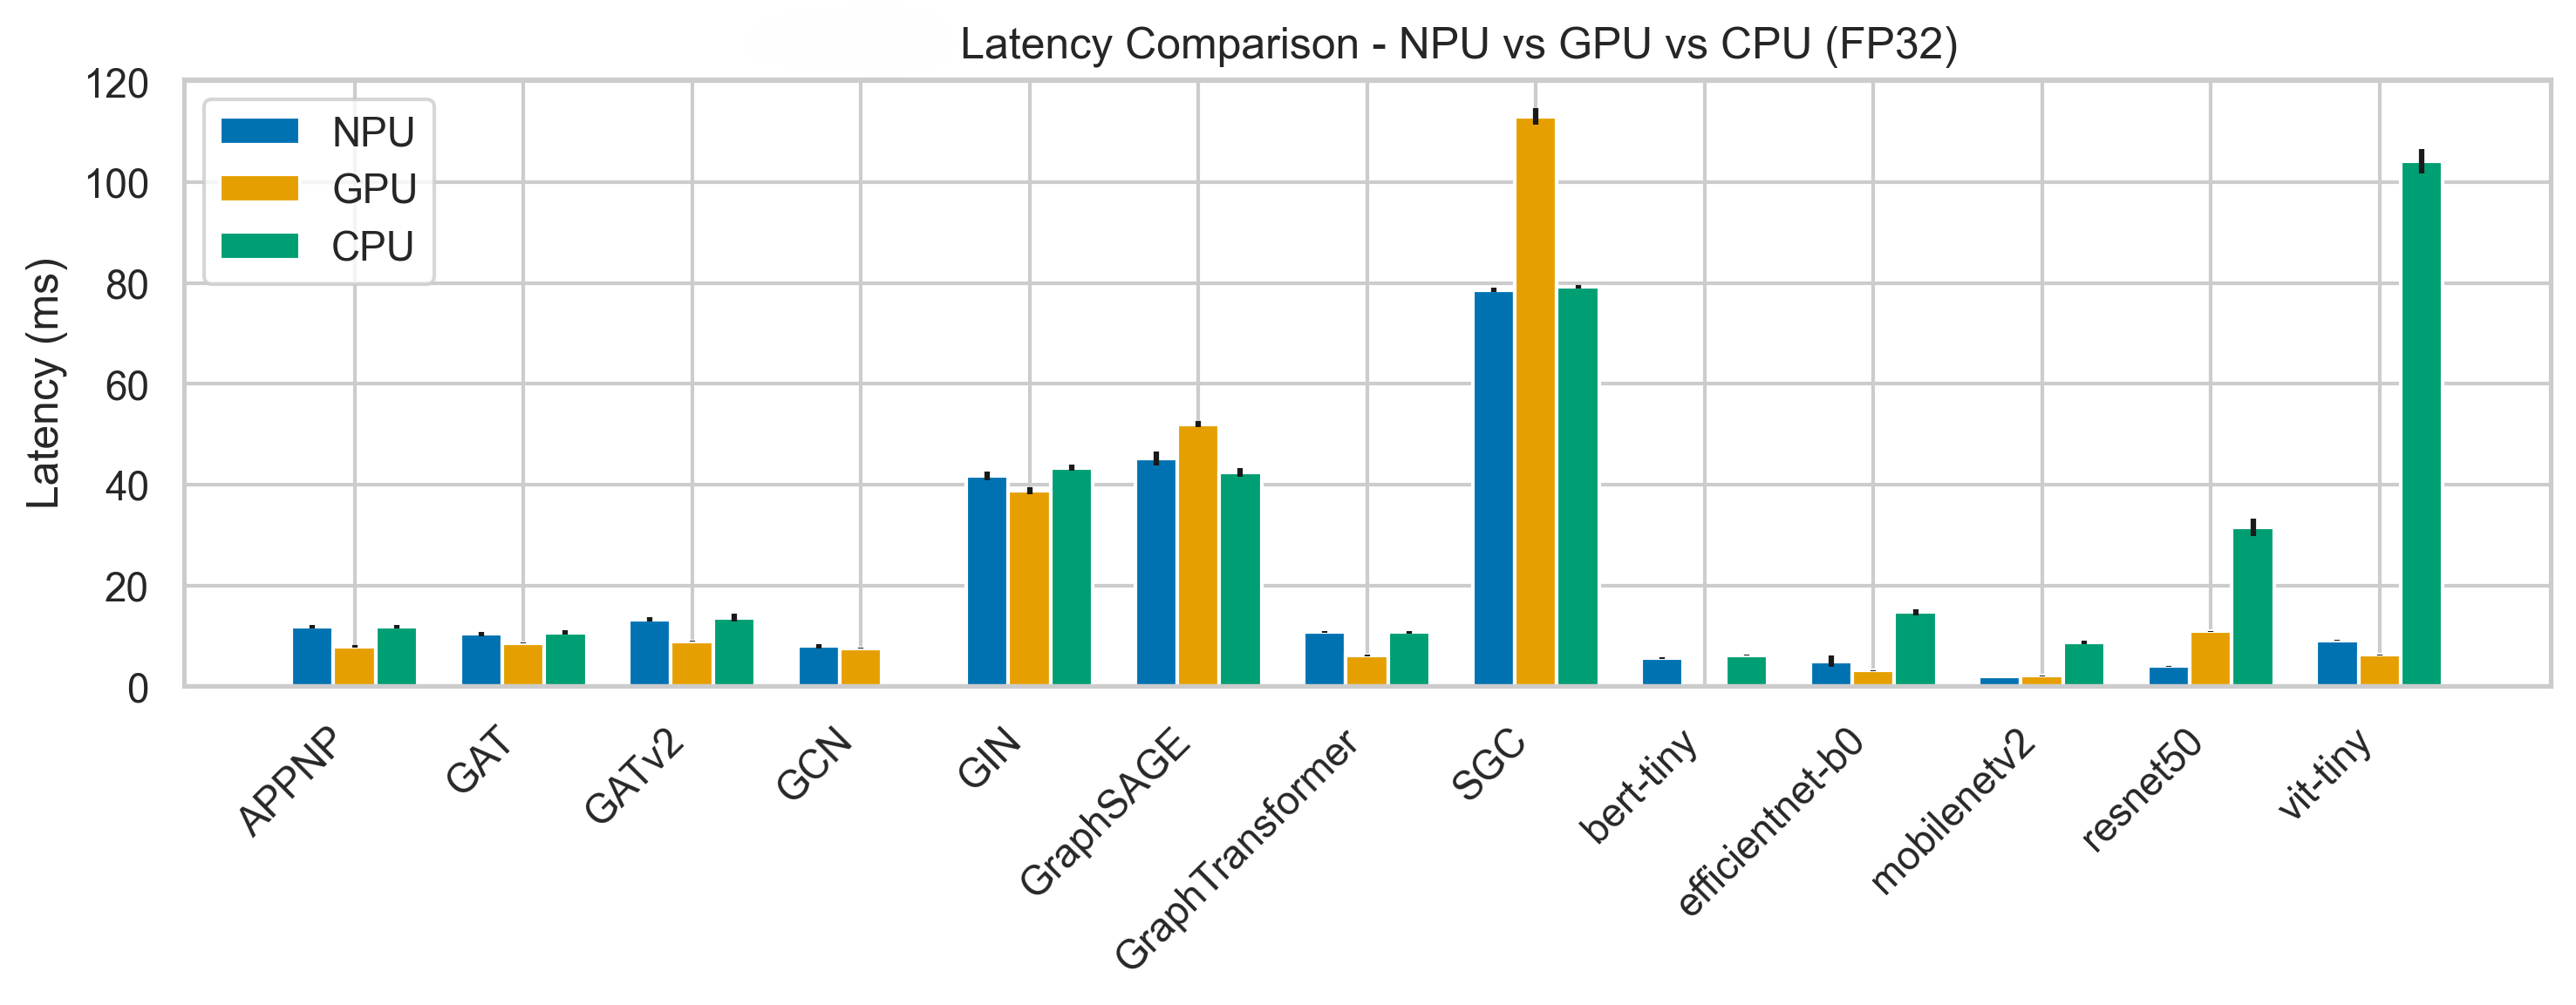
\includegraphics[width=0.74\columnwidth]{fig1_latency_comparison.png}
    \caption{FP32 latency comparison across CPU, iGPU, and NPU backends. Error bars indicate per-iteration standard deviation. GNNs show near-parity across backends; dense vision models exhibit significant NPU advantage.}
    \label{fig:fig1}
\end{figure}

\subsection{INT8 Quantization: Performance Impact}
Table~\ref{tab:int8} shows INT8 speedups on the NPU. GraphTransformer benefits (1.21$\times$) due to dense attention kernels. Other GNNs show marginal speedups (GCN: 1.04$\times$, GIN: 1.03$\times$, GraphSAGE: 1.05$\times$), indicating quantization does not alleviate memory bottlenecks. APPNP (0.84$\times$) and SGC show regressions; SGC's INT8 latency (173.90\,ms) is 2.2$\times$ slower than FP32 (78.59\,ms, 0.45$\times$ speedup) due to dispatch overhead during $K$-step propagation.
Dense vision models experience silent CPU fallback. MobileNetV2 INT8 on the NPU runs at 5.38\,ms (0.35$\times$ speedup) compared to 1.90\,ms in FP32; this matches its CPU INT8 latency of 5.46\,ms, indicating silent CPU fallback. Profiling confirms partial CPU dispatch for BERT-Tiny INT8 (154--231\,$\mu$s CPU execution) and ResNet50 (4.98\,ms NPU INT8 vs. 18.50\,ms CPU INT8). EfficientNet-B0 fails compilation (.failed marker) due to NPU incompatibility with per-channel dynamic quantization patterns.

\begin{table}[htbp]
\caption{INT8/FP32 Speedup on NPU (mean across OGB datasets)}
\begin{center}
\begin{tabular}{lccc}
\toprule
\textbf{Model} & \textbf{FP32 (ms)} & \textbf{INT8 (ms)} & \textbf{Speedup} \\
\midrule
GraphTransformer & 10.72 & 8.90 & \textbf{1.21$\times$} \\
GCN               & 7.91  & 7.58  & \textbf{1.04$\times$} \\
GraphSAGE         & 45.21 & 42.95 & 1.05$\times$ \\
GIN               & 41.68 & 40.55 & 1.03$\times$ \\
APPNP             & 11.75 & 13.96 & 0.84$\times$ \\
SGC               & 78.59 & 173.90 & 0.45$\times$ \\
\midrule
GAT               & 10.32 & --- & ---$^{\dagger}$ \\
GATv2             & 13.19 & --- & ---$^{\dagger}$ \\
\bottomrule
\end{tabular}
\label{tab:int8}
\end{center}
\footnotesize{Speedup $>$ 1.0 indicates INT8 faster. $^{\dagger}$INT8 compilation failed due to unsupported dynamic scatter/gather operations. EfficientNet-B0 also fails INT8. Vision models omitted due to evidence of NPU$\rightarrow$CPU fallback under INT8 (see text).}
\end{table}

\begin{figure}[htbp]
    \centering
    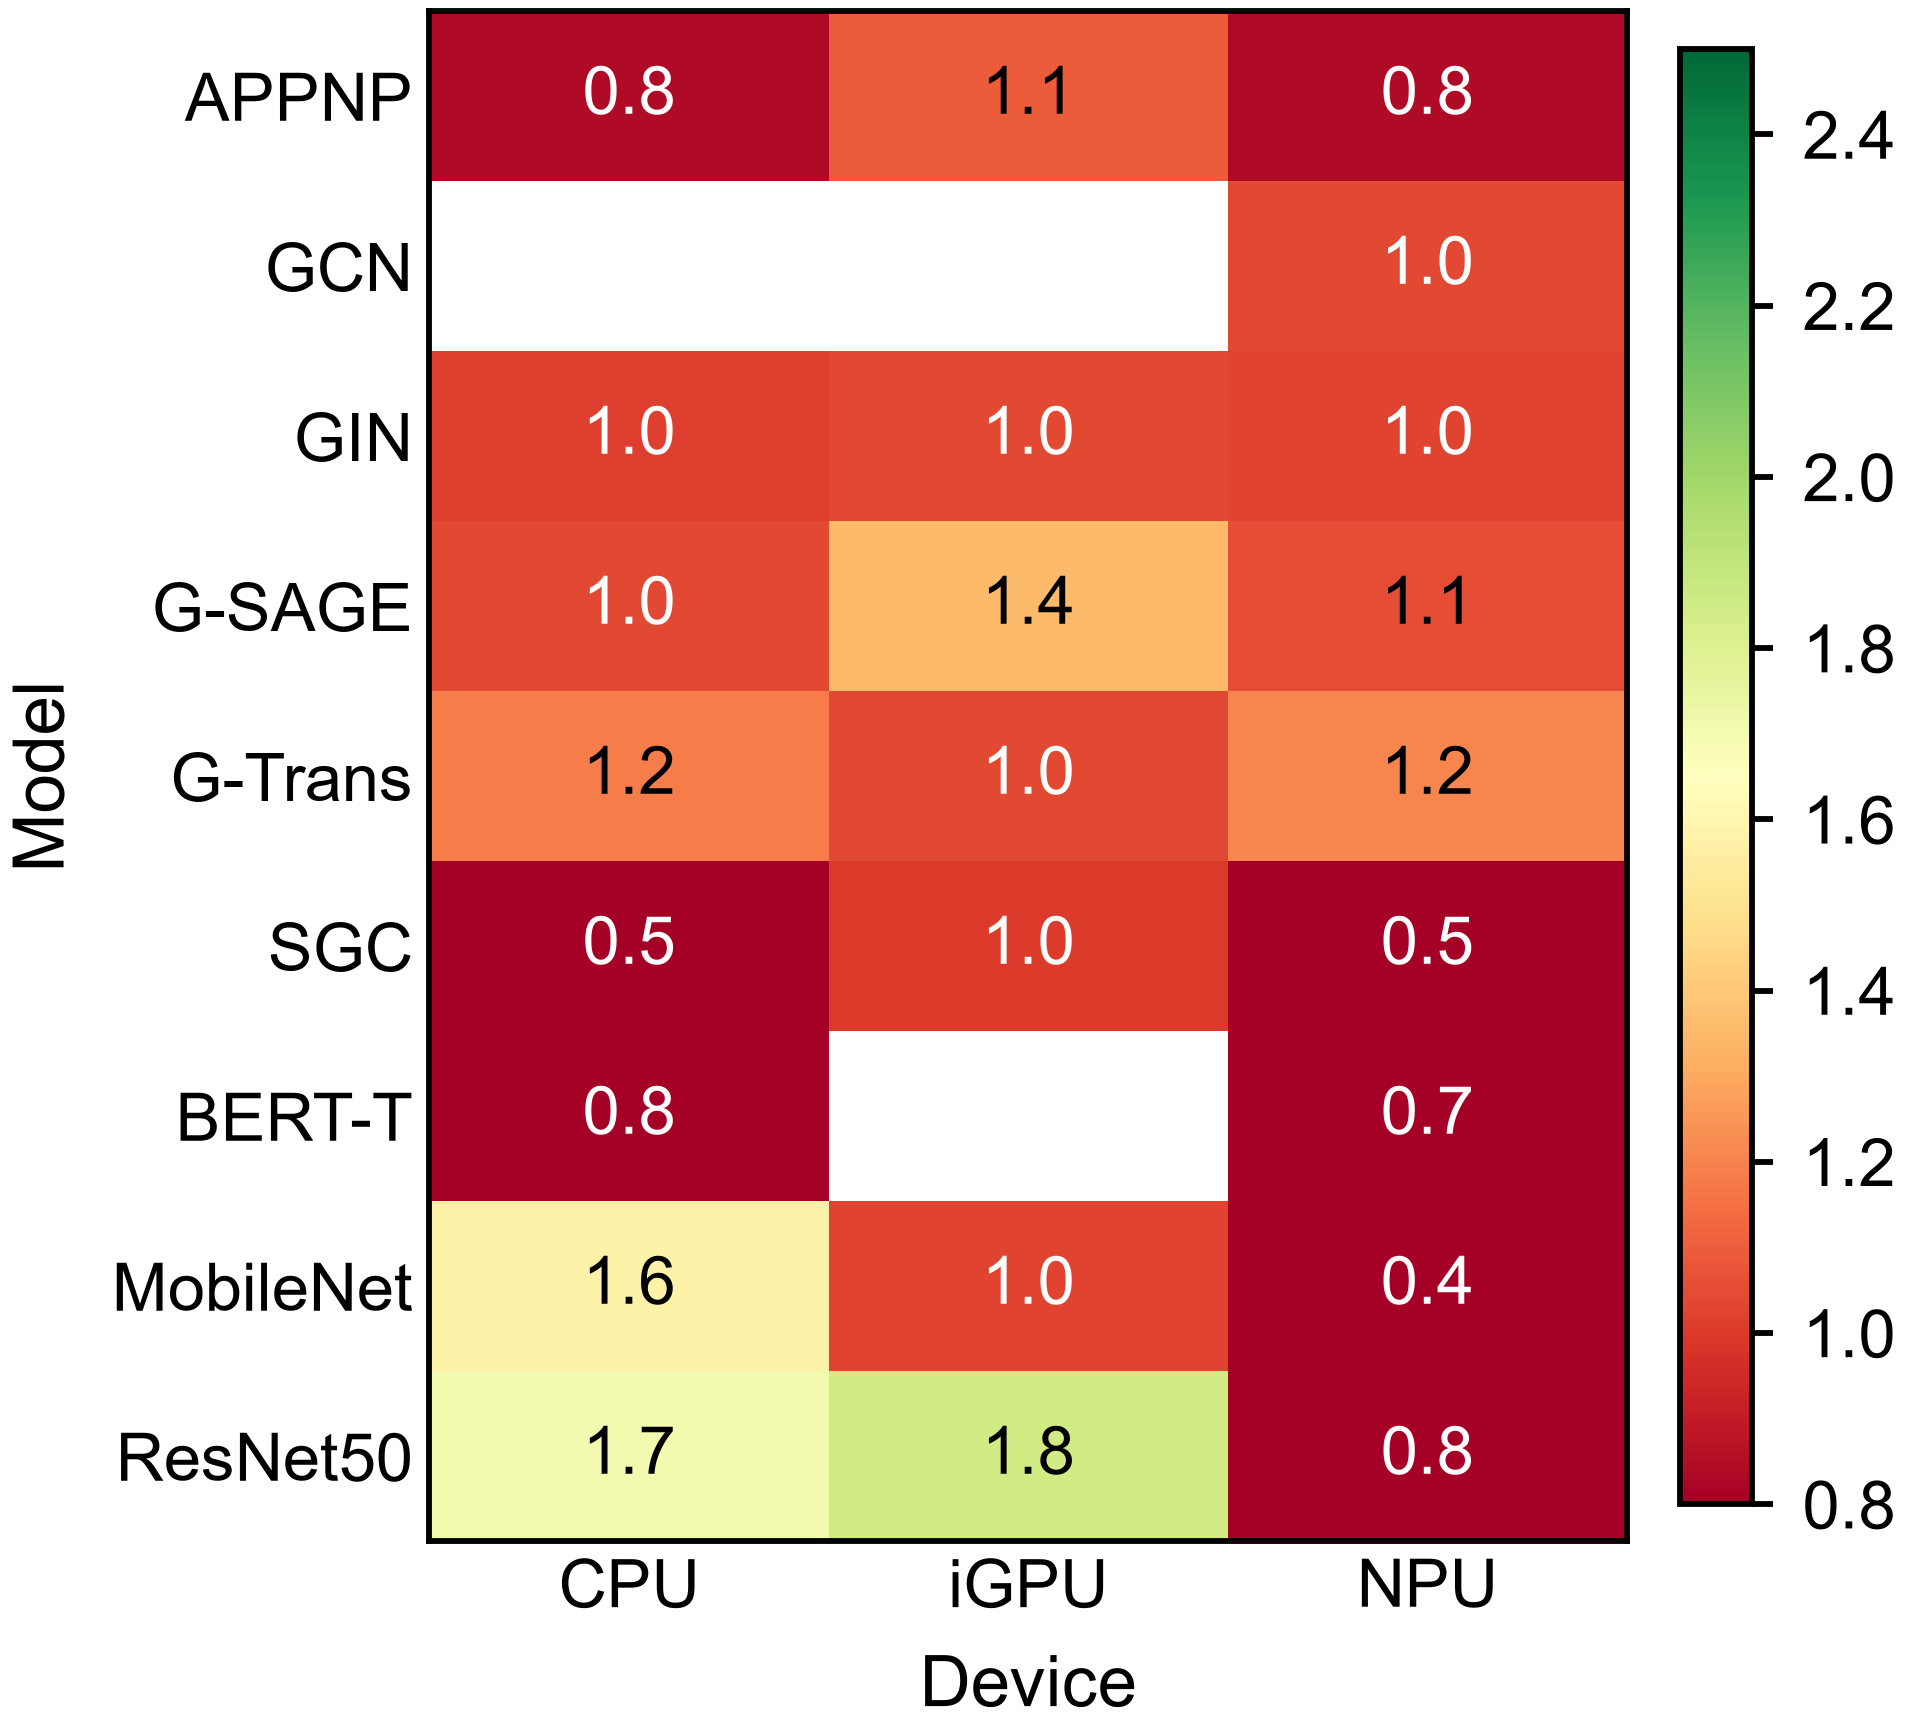
\includegraphics[width=0.74\columnwidth]{fig2_int8_speedup_heatmap.png}
    \caption{INT8 speedup heatmap across models and devices. Values below 1.0 (red) indicate INT8 regression. GPU consistently benefits; NPU and CPU show mixed results.}
    \label{fig:fig2}
\end{figure}

\subsection{Operator Composition Analysis}
Fig.~\ref{fig:fig3} illustrates operator breakdowns. GNNs are dominated by SpMM/MatMul/Gemm (30--60\% of nodes) and shape-manipulation primitives (Gather, Scatter, Reshape, Concat). Vision models consist mainly of Conv operations (50--80\%) with minimal shape manipulation.
While ViT-Tiny (5.7M parameters) achieves 11.4$\times$ speedup via structured, predictable attention maps, GraphTransformer (0.18M parameters) gains no NPU speedup (10.72\,ms NPU vs. 10.69\,ms CPU) due to dynamic, irregular graph neighborhoods.

\begin{figure}[htbp]
    \centering
    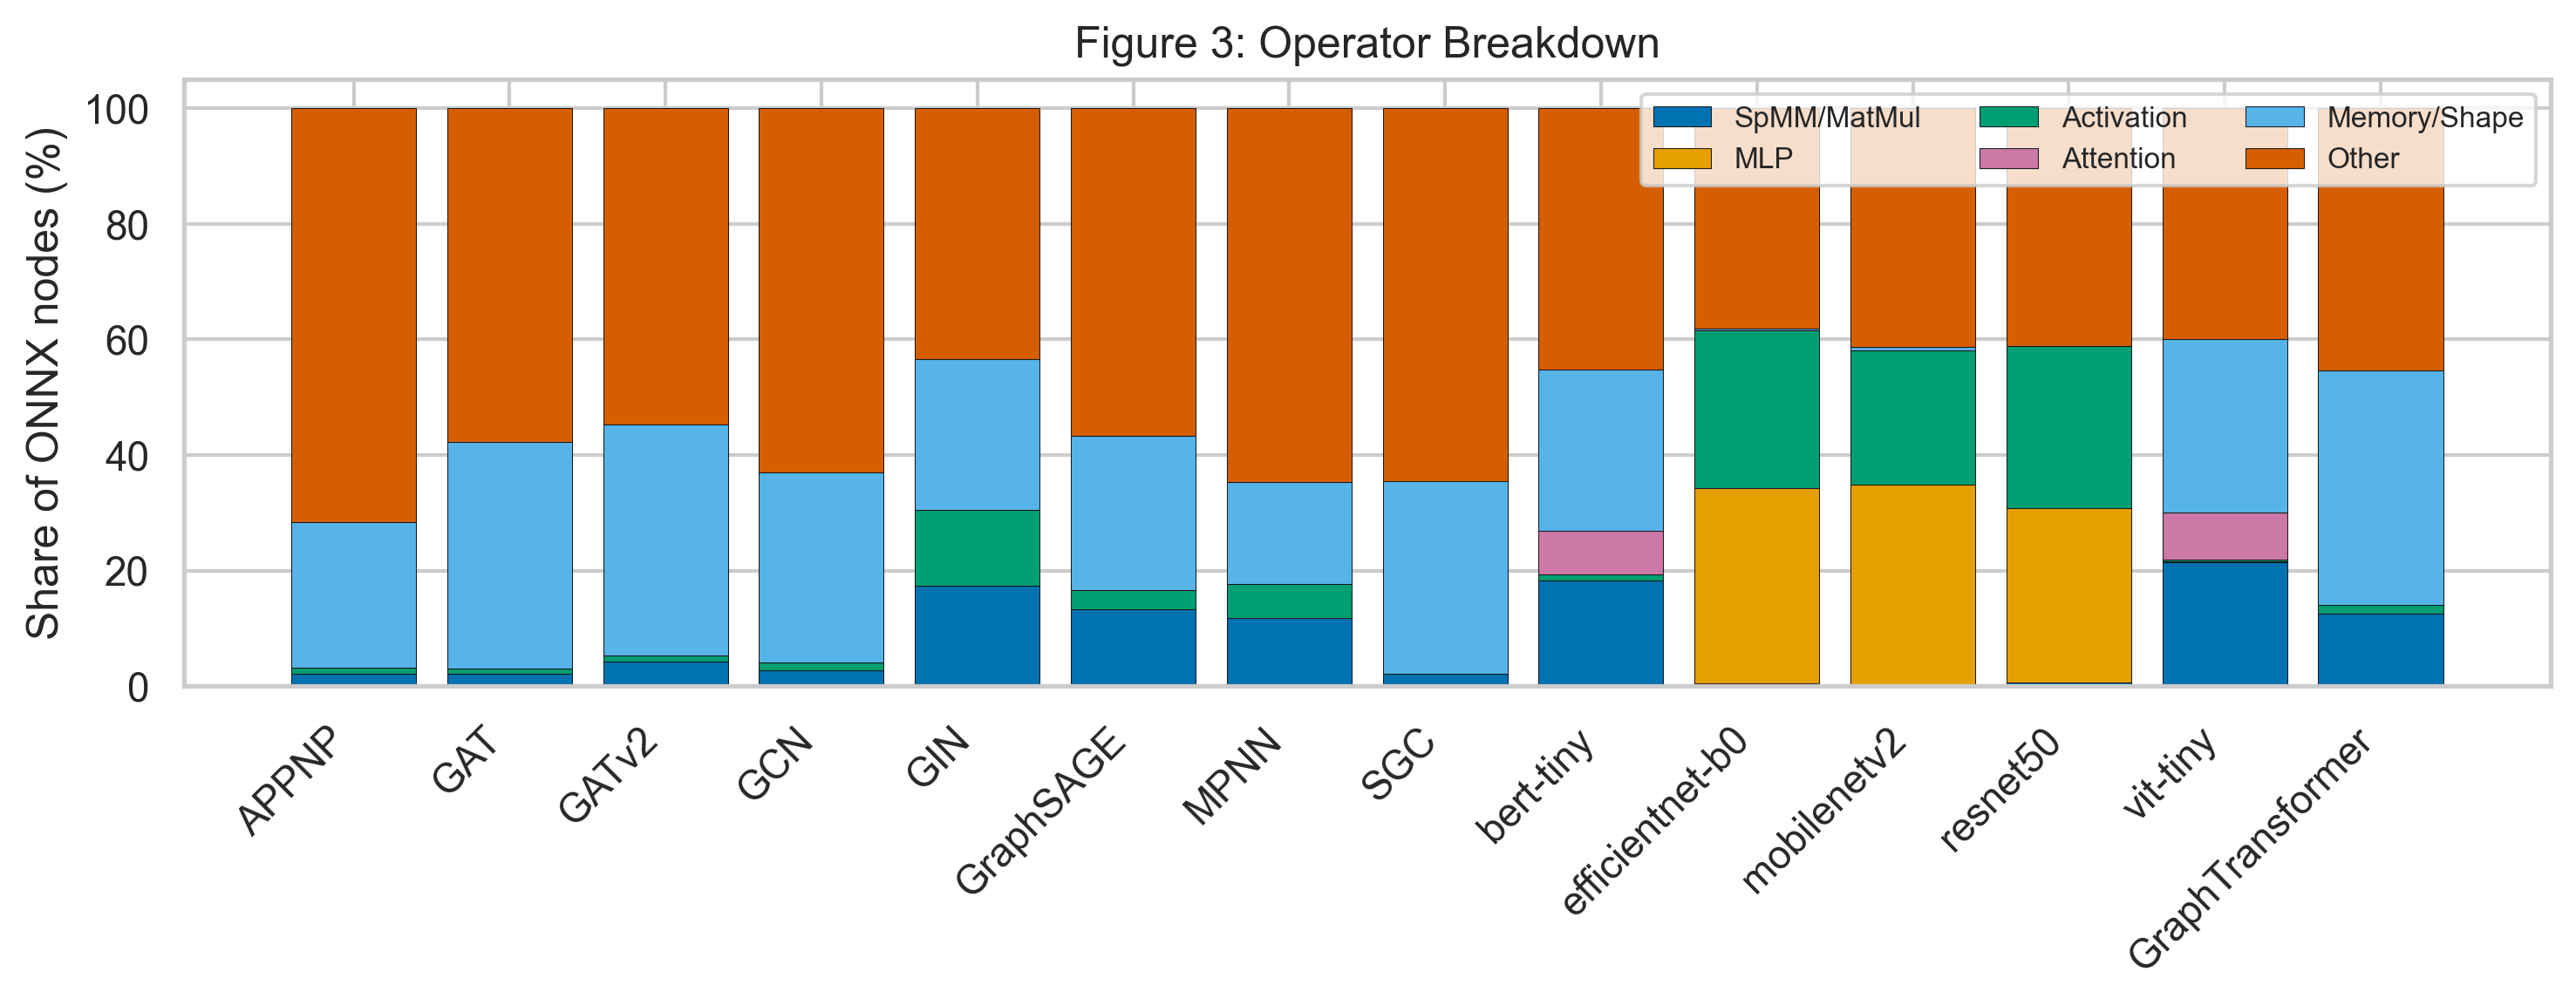
\includegraphics[width=0.74\columnwidth]{fig3_operator_breakdown.png}
    \caption{Operator composition of FP32 models. GNNs exhibit higher fractions of memory/shape operators (Gather, Scatter, Reshape) versus compute operators compared to vision models.}
    \label{fig:fig3}
\end{figure}

\subsection{CPU Fallback and Operator Coverage}
Fig.~\ref{fig:fig4} profiles the CPU fallback fractions. Most GNN operations compile natively (0\% fallback), and BERT-Tiny fallback is restricted to embedding lookups (0.5\% time). However, MPNN exhibits 100\% fallback to CPU (producing zero NPU entries in the scalability matrix) due to unsupported \texttt{index\_add\_} and \texttt{scatter\_mean} operators. GAT, GATv2, and EfficientNet-B0 fail INT8 compilation, producing \texttt{.failed} markers. The toolchain does not quantize the attention-related Gather/Scatter and MBConv operators, and the dynamic quantization API restricts fine-grained per-operator mitigation.

\begin{figure}[htbp]
    \centering
    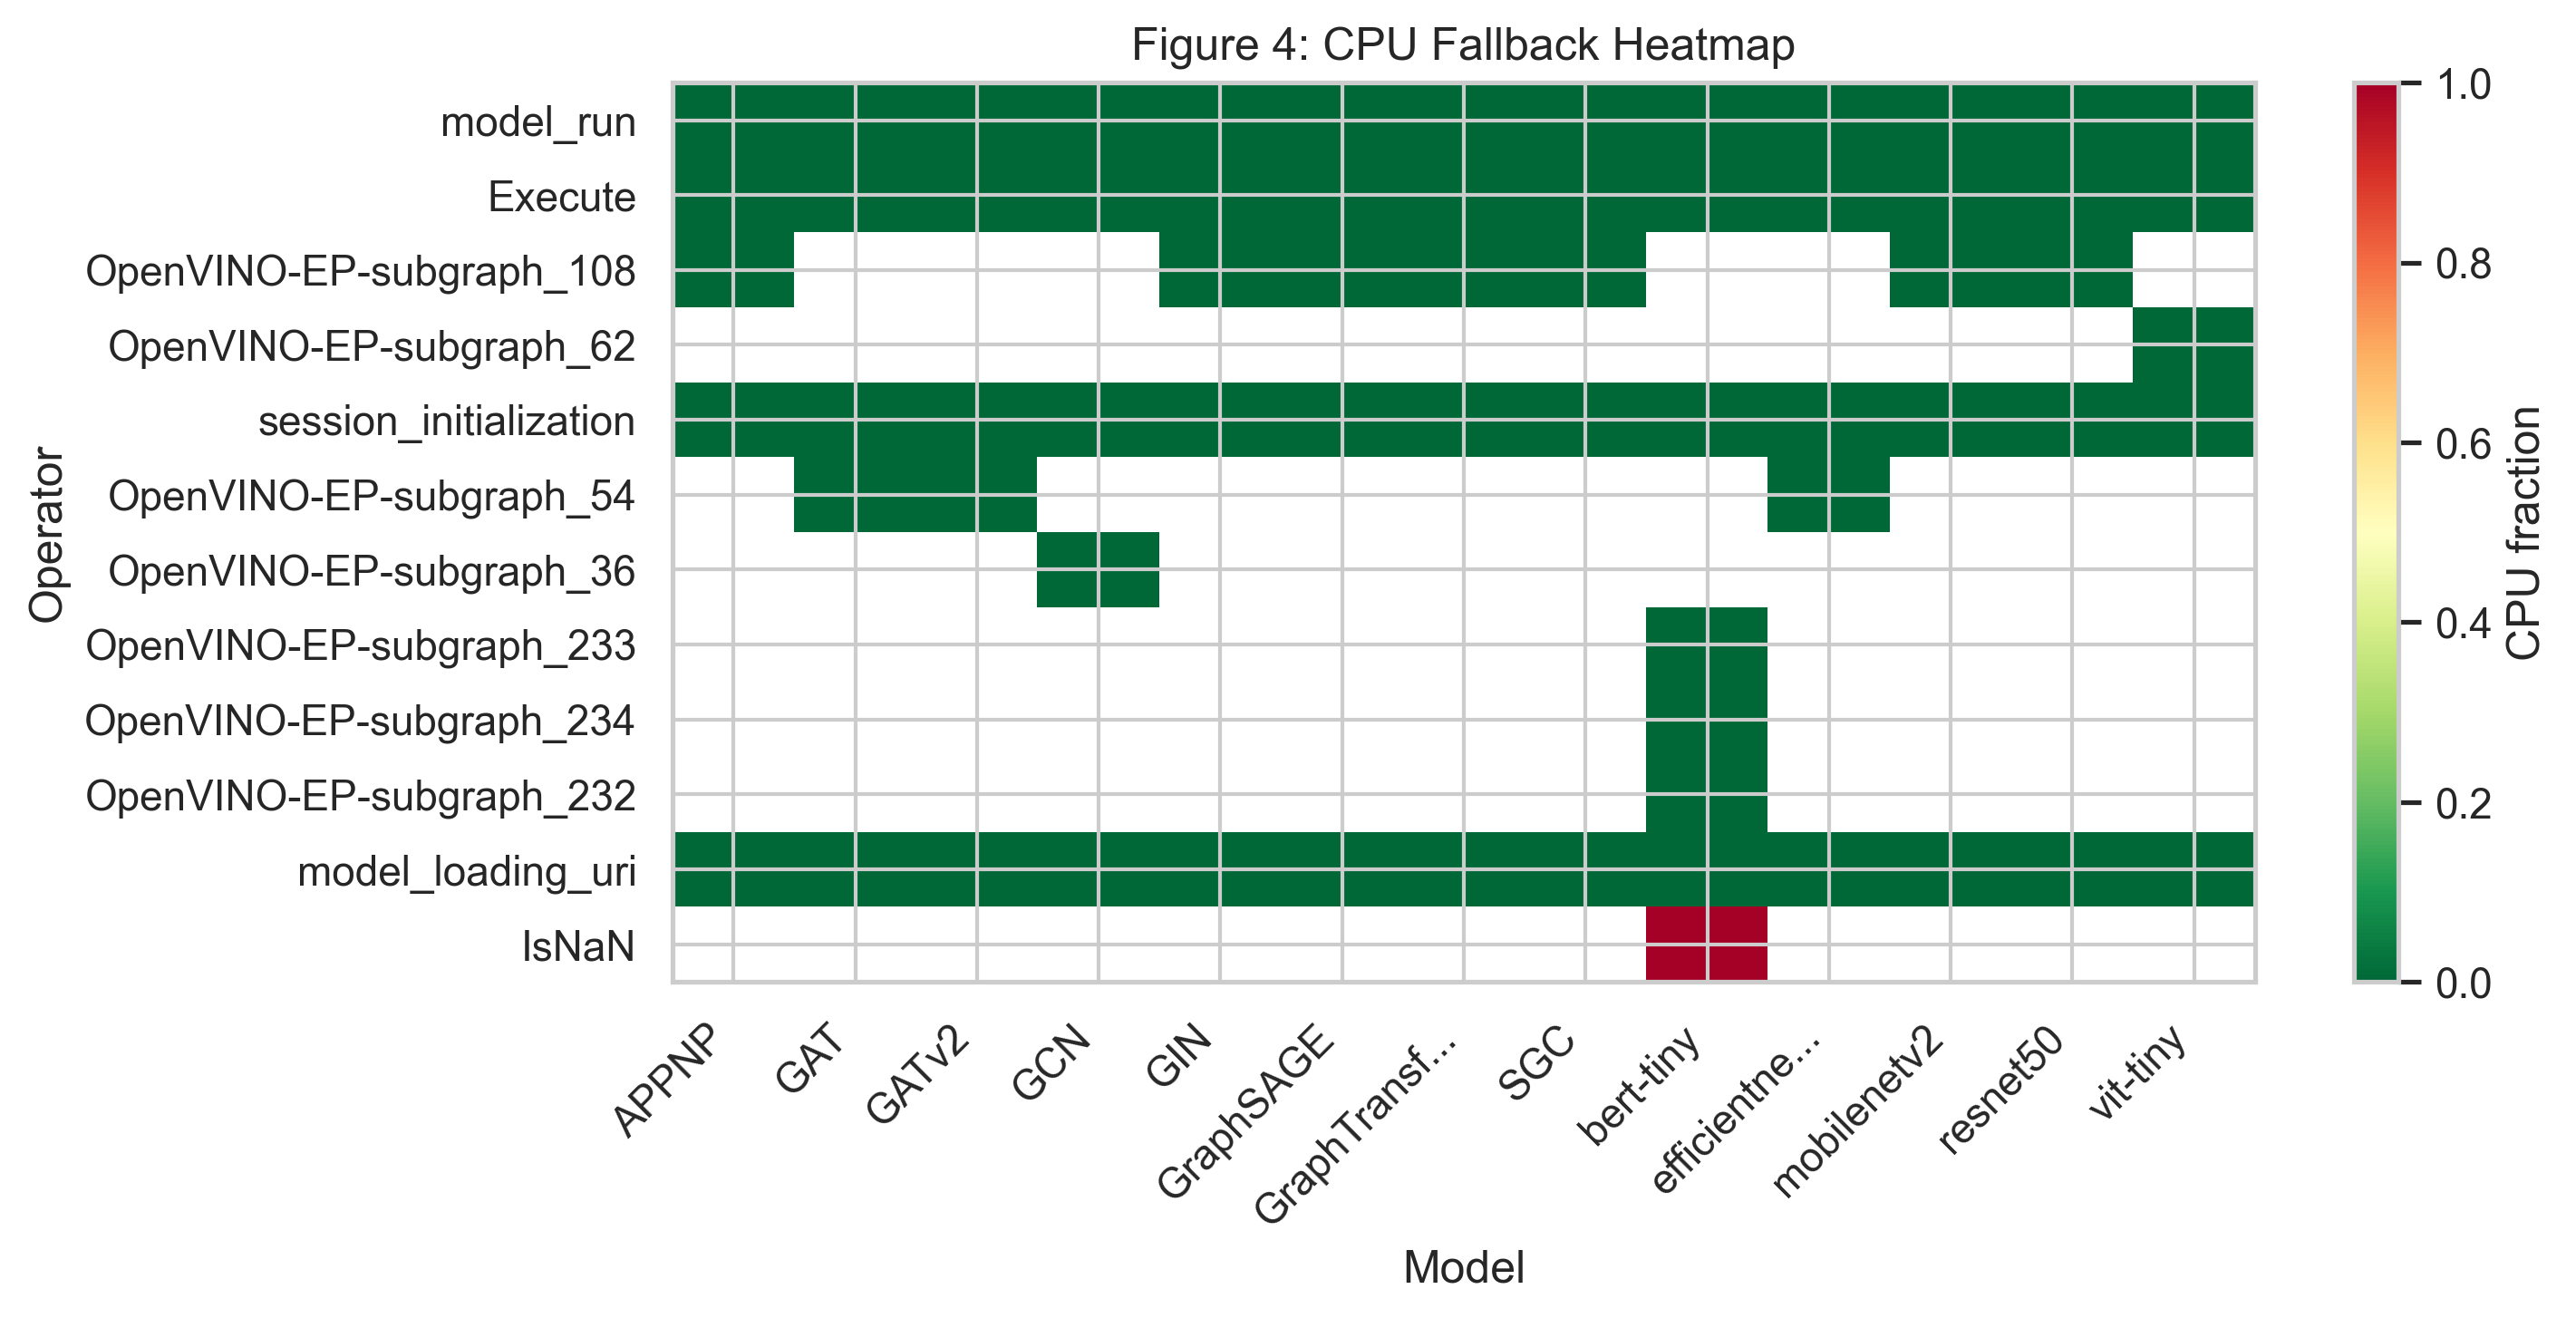
\includegraphics[width=0.74\columnwidth]{fig4_cpu_fallback_heatmap.png}
    \caption{CPU fallback fraction per operator across models. Most operators run natively on the assigned backend. MPNN and attention-based models trigger toolchain limitations.}
    \label{fig:fig4}
\end{figure}

\subsection{Optimization Speedup and Roofline Analysis}
Fig.~\ref{fig:fig5a} shows optimization speedups (extended vs. disabled ORT). NPU optimization gains are small (1.0--1.05$\times$), whereas GPU optimization achieves 1.1--1.25$\times$ speedup via OpenVINO kernel fusion.
Fig.~\ref{fig:fig5b} presents a throughput-intensity roofline. GNNs cluster in the low-intensity (0.1--10 FLOP/byte) and low-throughput (1--3\,GFLOP/s) region, well below the platform peak LPDDR5x bandwidth ceiling (120\,GB/s). In contrast, ResNet50 and MobileNetV2 utilize the NPU's compute pipelines more effectively (8--20\,GFLOP/s at 18--72 FLOP/byte). The NPU's effective bandwidth ceiling is estimated at 50--60\,GB/s due to shared SoC fabric contention \cite{lam2024_meteorlake_npu}.

\begin{figure}[htbp]
    \centering
    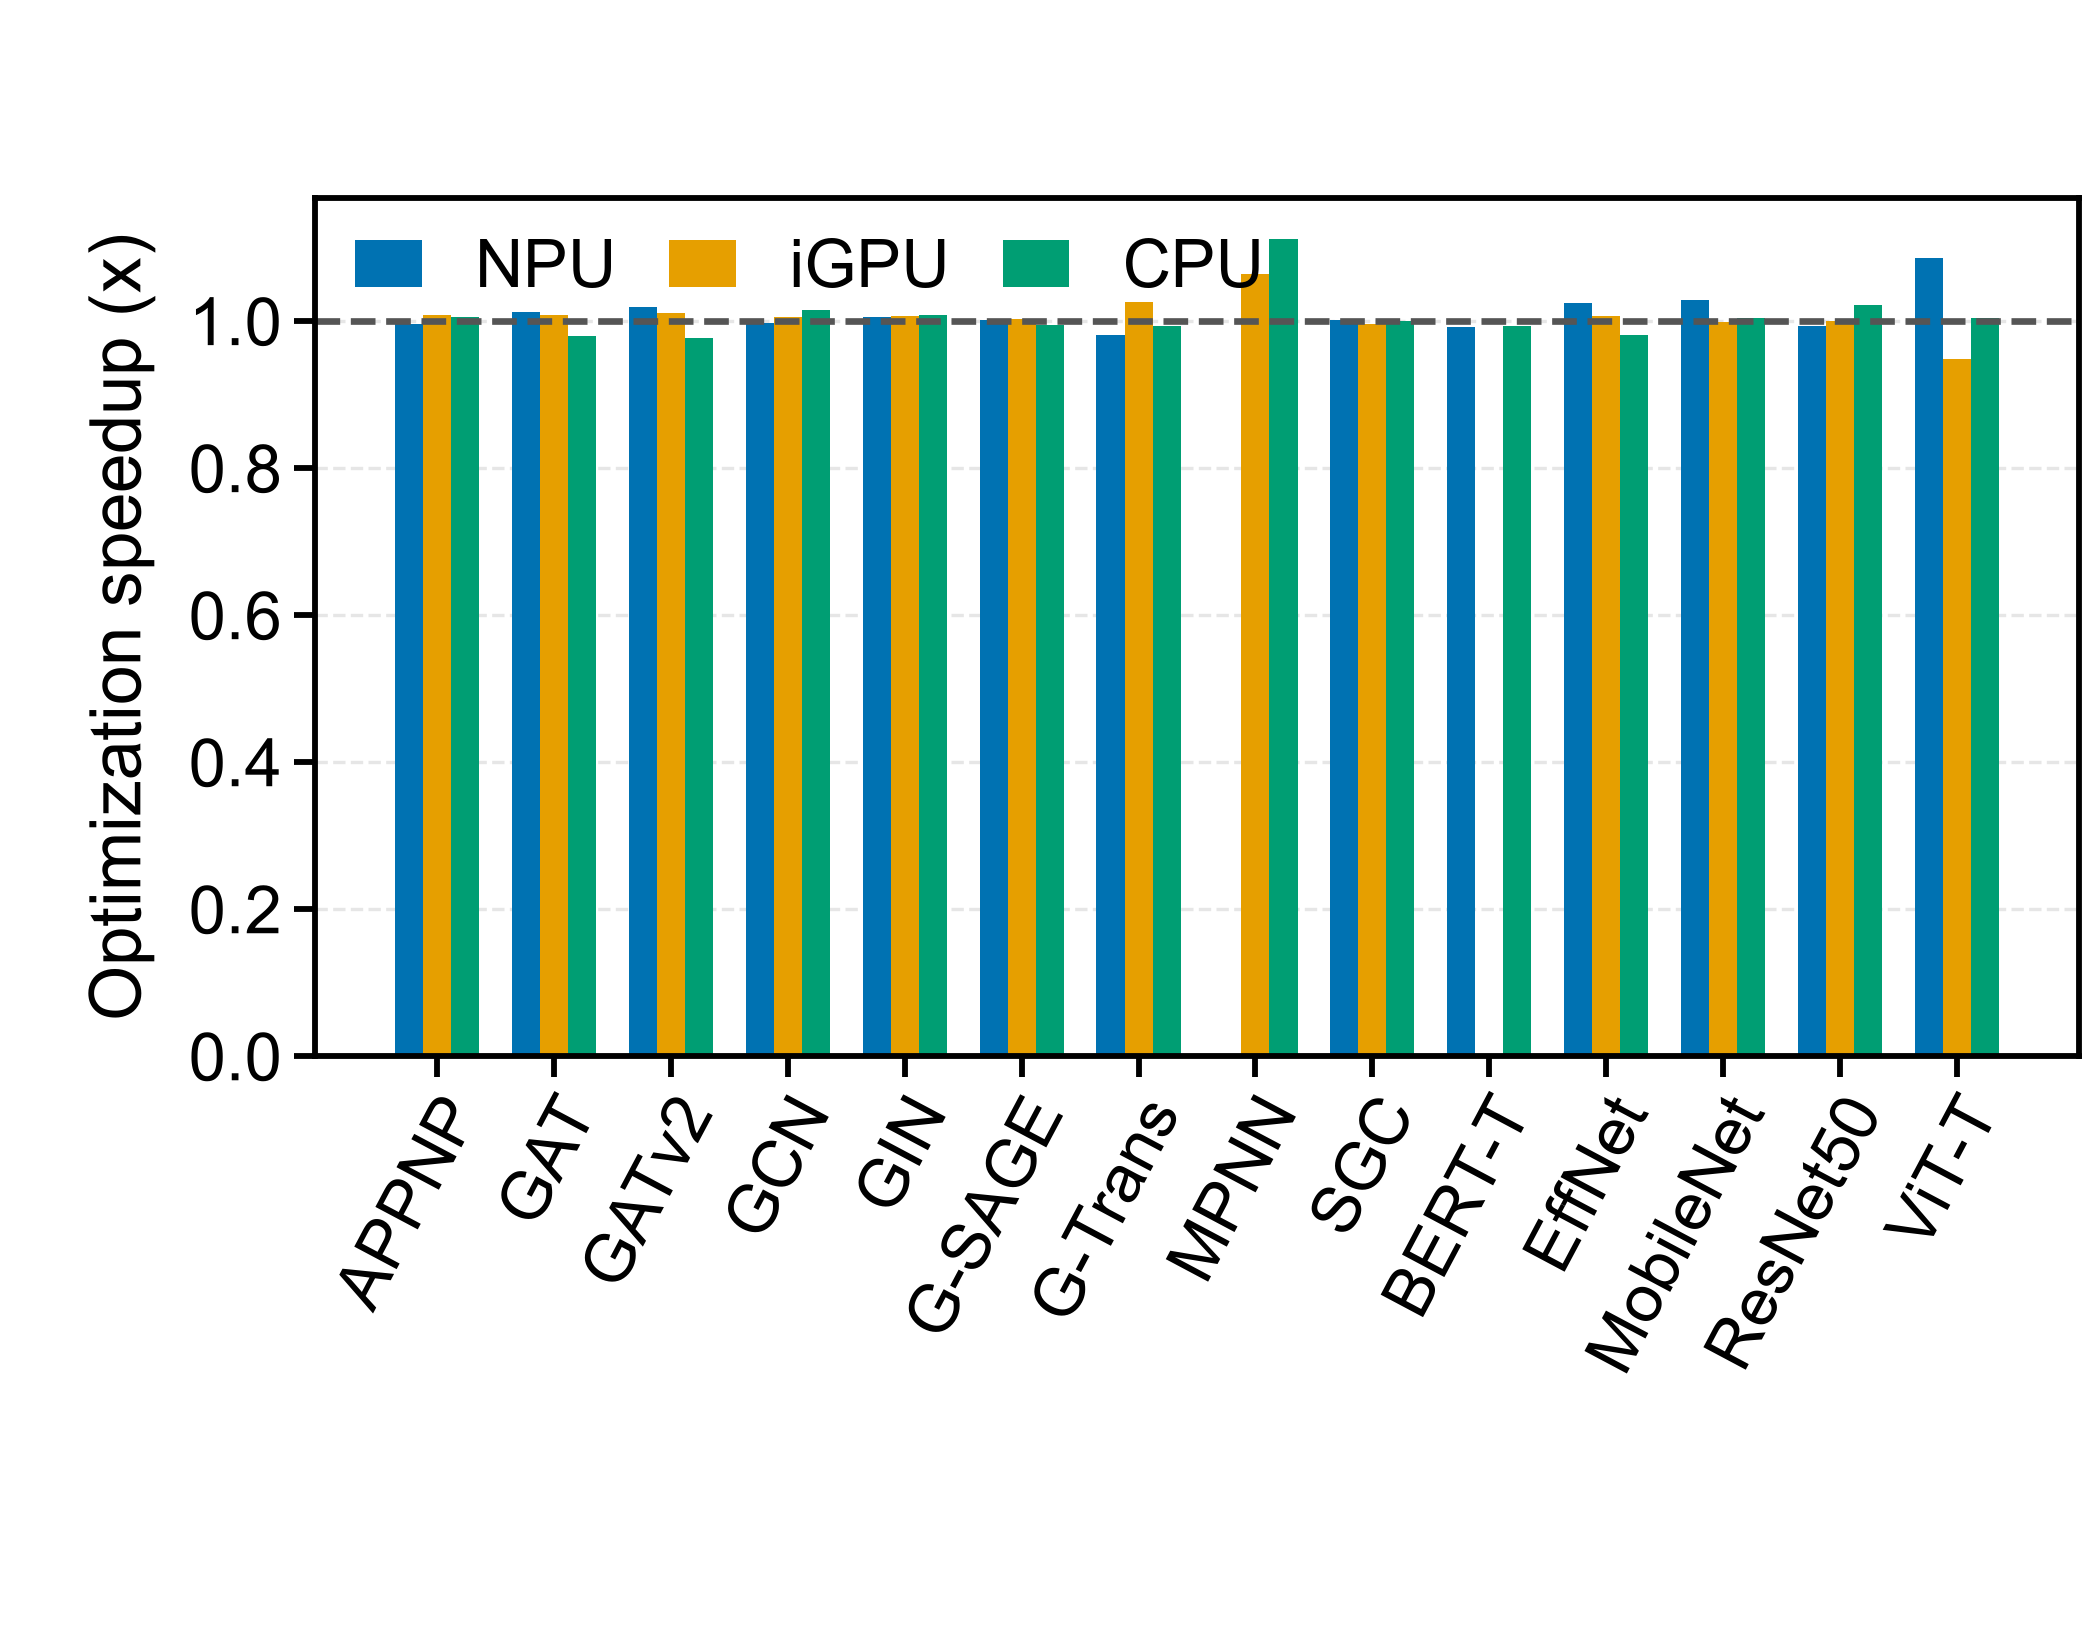
\includegraphics[width=0.74\columnwidth]{fig5a_opt_speedup.png}
    \caption{ORT optimization speedup by device. GPU shows larger gains from graph-level optimization for GNNs; NPU optimization returns are uniformly modest.}
    \label{fig:fig5a}
\end{figure}

\begin{figure}[htbp]
    \centering
    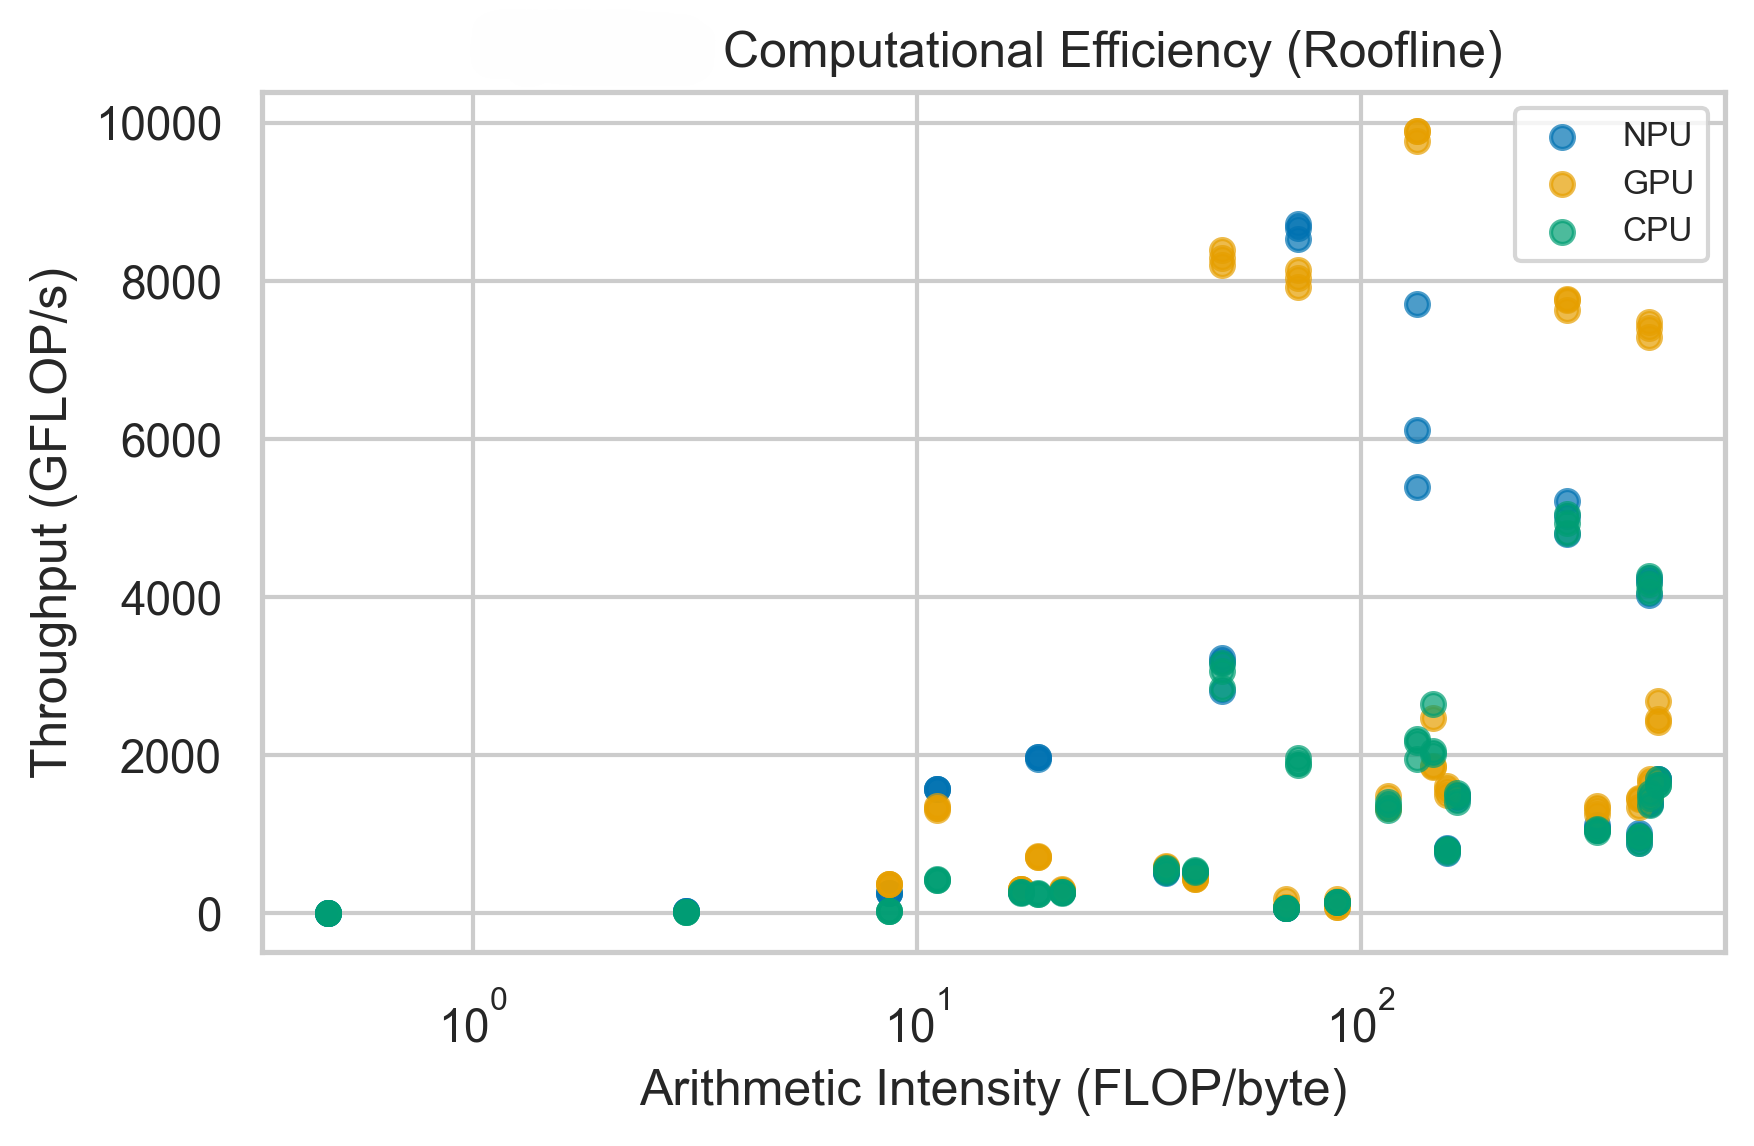
\includegraphics[width=0.74\columnwidth]{fig5b_roofline.png}
    \caption{Computational efficiency (throughput vs.\ arithmetic intensity). GNNs occupy the memory-bound region (low intensity, low throughput); vision models on NPU achieve higher operational intensity.}
    \label{fig:fig5b}
\end{figure}

\subsection{Graph Density, Scaling, and Static-Shape Compilation}
Figs.~\ref{fig:fig7} and~\ref{fig:fig6} analyze NPU latency versus graph density (6.9--451.7\,edges/node) and size. NPU latency is invariant to graph density ($r=-0.00$, $p=0.993$) or node count. This occurs because the toolchain compiles models with static shapes; the execution plan processes a fixed-size representation. While CPU and GPU latencies scale with input size, the static-shape NPU execution model prioritizes latency predictability over proportional density-dependent speedups.

\begin{figure}[htbp]
    \centering
    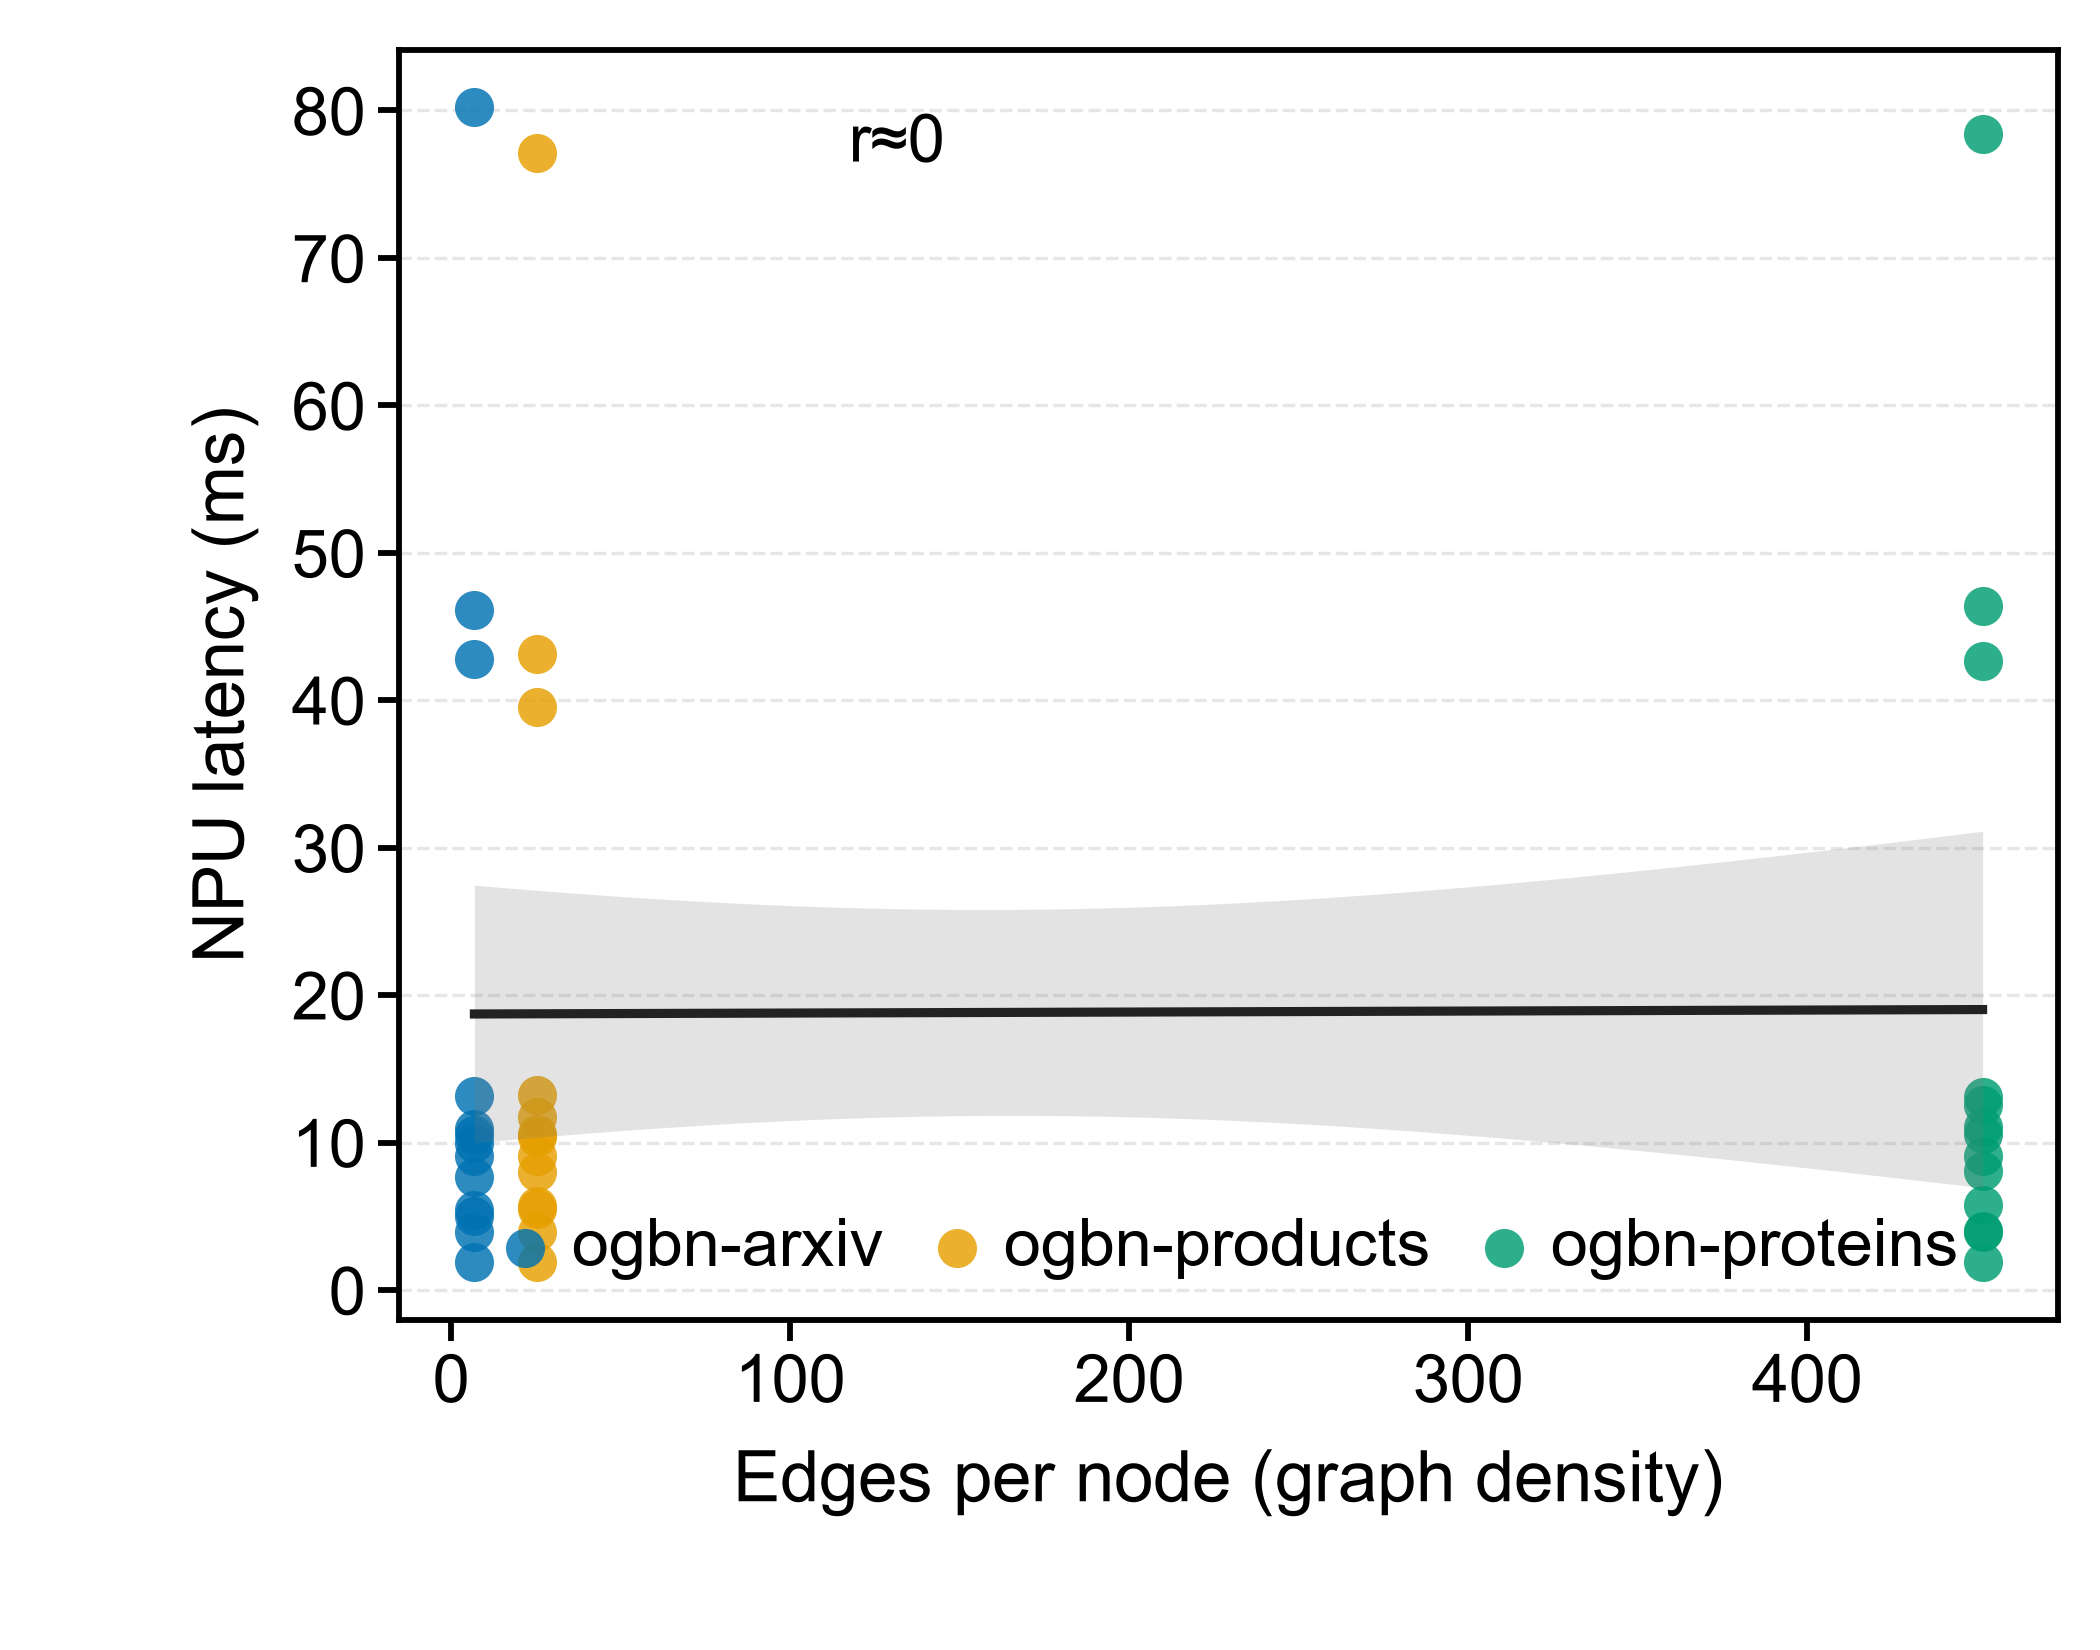
\includegraphics[width=0.74\columnwidth]{fig7_density_vs_latency.png}
    \caption{NPU latency vs.\ graph density. The flat regression line ($r\approx 0$) indicates static-shape compilation decouples inference time from input sparsity.}
    \label{fig:fig7}
\end{figure}

\begin{figure}[htbp]
    \centering
    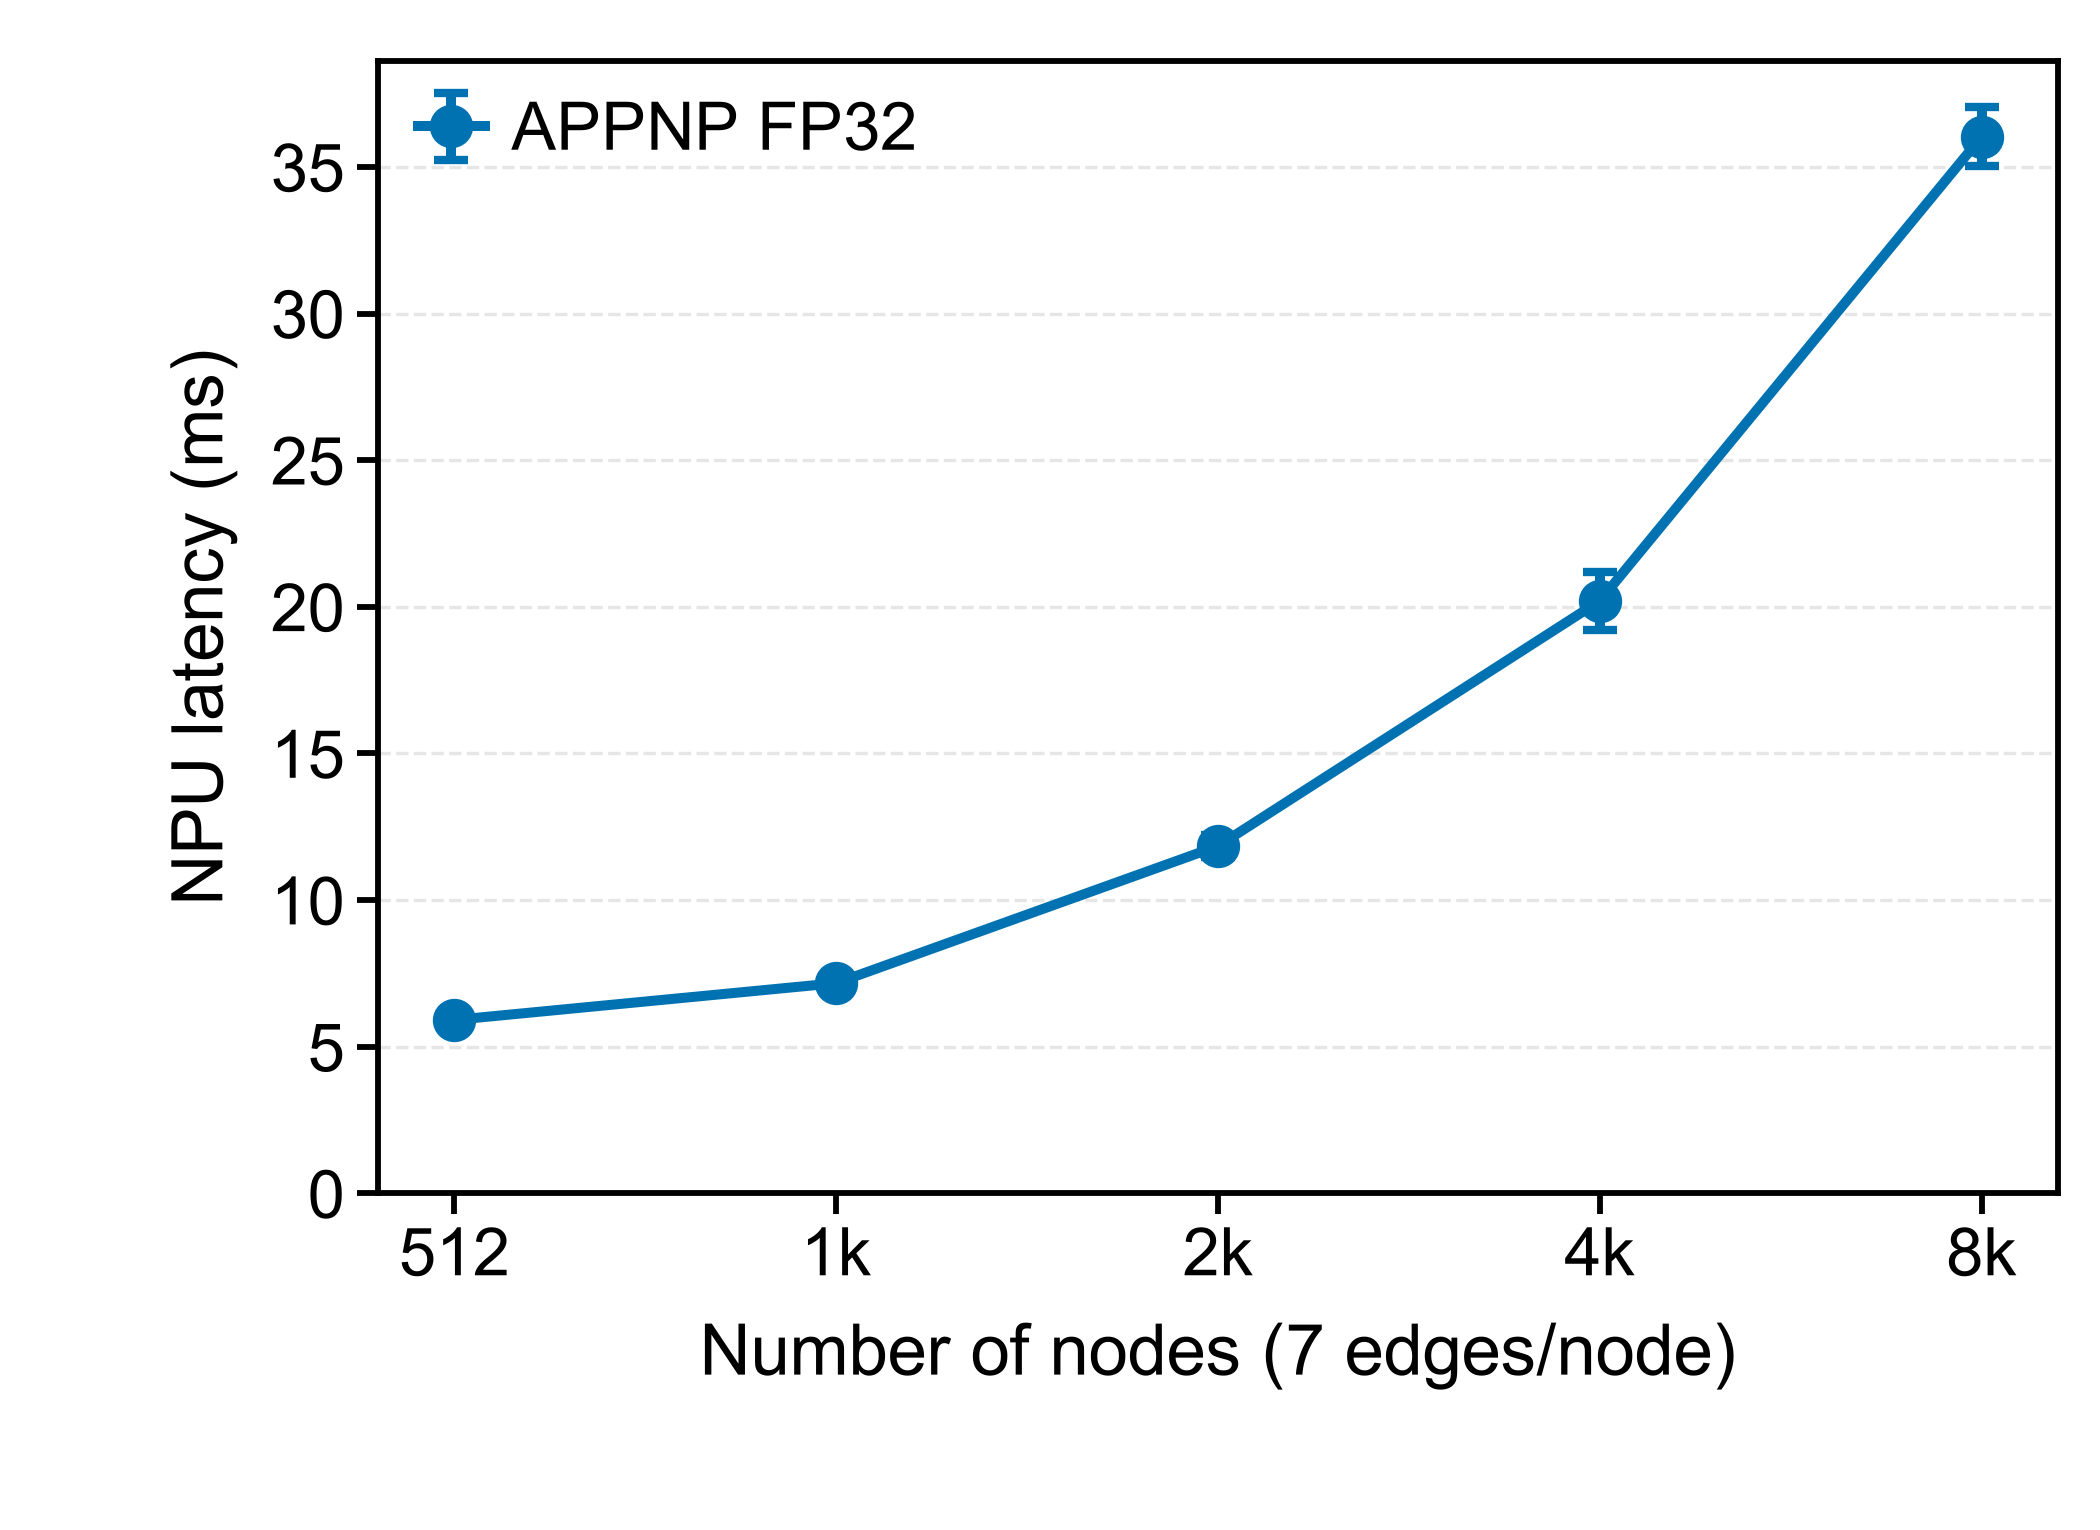
\includegraphics[width=0.74\columnwidth]{fig6_scaling.png}
    \caption{Scaling characteristics across models on NPU. Latency remains nearly constant across graph sizes due to static-shape compilation.}
    \label{fig:fig6}
\end{figure}

\subsection{Energy Consumption Analysis}
Table~\ref{tab:energy} shows package-level power collected via SoCWatch (\texttt{-f sys -t 30 -r sum}). The GPU draws higher power than the CPU for GCN (12,482\,mW vs. 11,629\,mW, +7.3\%) but reduces latency (6.94\,ms vs. 7.73\,ms), resulting in comparable energy per inference (86.6 vs. 89.9\,mJ). For MPNN, which falls back to the CPU, package power (9,357 vs. 9,473\,mW) and latencies (20.23 vs. 22.03\,ms) remain nearly identical.
CPU INT8 quantization for GCN reduces power (11,629 to 9,675\,mW, --16.8\%) with stable latency (7.73 to 7.59\,ms, --1.8\%), decreasing energy by 18.4\%. Conversely, MPNN CPU INT8 increases latency to 32.94\,ms (+63\% over FP32: 20.23\,ms) and energy to 301.1\,mJ (+59\% over FP32: 189.3\,mJ), despite a slight power decrease (9,139 vs. 9,357\,mW). For GNNs, INT8 energy benefits are model-dependent and not guaranteed. NPU power rail isolation was unavailable under the current PMT interface.

\begin{table}[htbp]
\caption{Package Power and Energy per Inference (SoCWatch, 30\,s collection window)}
\begin{center}
\begin{tabular}{llrrr}
\toprule
\textbf{Model} & \textbf{Config} & \textbf{Avg Power} & \textbf{Latency} & \textbf{Energy/Inf.} \\
 & & \textbf{(mW)} & \textbf{(ms)} & \textbf{(mJ)} \\
\midrule
\rowcolor{gray!15} GCN & CPU FP32 & 11,629 & 7.73 & 89.9 \\
GCN & CPU INT8 & 9,675 & 7.59 & 73.4 \\
\rowcolor{gray!15} GCN & GPU FP32 & 12,482 & 6.94 & 86.6 \\
\midrule
\rowcolor{gray!15} MPNN & CPU FP32 & 9,357 & 20.23 & 189.3 \\
MPNN & CPU INT8 & 9,139 & 32.94 & 301.1 \\
\rowcolor{gray!15} MPNN & GPU FP32 & 9,473 & 22.03 & 208.7 \\
MPNN & GPU INT8 & 9,161 & 32.48 & 297.6 \\
\bottomrule
\end{tabular}
\label{tab:energy}
\end{center}
\footnotesize{Latency is the mean time over 100 iterations $\times$ 3 repeats across three OGB datasets. Energy/inf.\ is estimated as \(\text{Avg Power} \times \text{Mean Latency}\) over the 30\,s SoCWatch window, representing an upper bound that includes background system activity. NPU power isolation was unsupported by the PMT interface.}
\end{table}

\section{Discussion}

\subsection{Why INT8 Fails for GNNs on NPU}
The low performance gains of INT8 quantization for GNNs on the Meteor Lake NPU stem from a combination of hardware memory constraints, quantization mismatches, and software compiler limitations.

First, GNN execution is memory-bound; SpMM latency is dominated by fetching irregularly indexed feature vectors from DRAM rather than raw arithmetic. Reducing precision to INT8 lowers compute latency but does not alleviate the memory bandwidth bottleneck. Second, the NPU's quantization pipeline is optimized for per-tensor symmetric quantization of convolutional weights. For GNNs, per-channel weight distributions and dynamic activation ranges from varying graph structures trigger significant dequantization overhead or fallback to the CPU. This is compounded by the fact that GNNs contain 2--4$\times$ more shape-manipulation operators (Gather, Scatter, Reshape) than vision models, which are poorly served by uniform quantization.

At the compiler level, the OpenVINO toolchain applies fewer fusion optimizations to GNNs than to CNNs. Aggressive kernel fusion relies on consecutive memory access patterns, which are broken in GNNs by the indirect indexing of sparse operations \cite{10.1145/3453483.3454083}. Specifically, the compiler cannot merge a Gather operation (indexing vertex features) with a subsequent MatMul because the intermediate data layouts are determined dynamically at runtime by the input graph adjacency. Consequently, the compiler fails to generate fused execution blocks, leaving the NPU to stall on discrete DRAM reads while receiving fewer optimization passes from the software stack.

Finally, the NPU's failure mode under unsupported quantized operators involves silent CPU fallback rather than compile-time termination. This behavior, observed for MobileNetV2, ResNet50, and BERT-Tiny INT8, masks execution bottlenecks by transparently dispatching unsupported operators to the CPU. Unless practitioners actively monitor CPU-fallback ratios, this silent dispatch yields misleading latency profiles. While future compiler updates may improve quantized operator coverage or support explicit mixed-precision, the fundamental memory-bandwidth limit will persist for streaming-dataflow accelerators lacking native sparse-dataflow hardware engines.

\subsection{Platform Maturity Assessment}
Under OpenVINO 2024.1, the Meteor Lake NPU acts primarily as a vision-centric accelerator. Dense convolutional models achieve 4.5--11.4$\times$ speedups over the CPU (MobileNetV2: 4.5$\times$, ResNet50: 8.0$\times$, ViT-Tiny: 11.4$\times$) at low TDP. In contrast, for GNN workloads, CPU and GPU backends run in a 9.1--12.5\,W package power range, with the GPU drawing 7.3\% more power for GCN while maintaining similar latency. NPU GNN support is restricted by incomplete operator coverage (e.g., MPNN CPU fallback), unreliable quantization, and a memory subsystem not optimized for sparse, irregular access patterns.
The iGPU's latency advantage over the NPU for GNNs is driven by: (1) higher effective memory bandwidth (128-bit LPDDR5x interface vs. shared SoC fabric), (2) a larger cache (4--8\,MB L2 vs. the NPU's small SRAM), and (3) more effective kernel fusion under the OpenVINO GPU plugin (1.1--1.25$\times$ speedup vs. 1.0--1.05$\times$ on the NPU). Because GNNs are memory-bound (Section~IV-E), memory bandwidth and cache sizes directly limit performance. These hardware constraints align with findings that GNNs are not always optimal for sparse graph problems \cite{Bayraktar2026}.

\subsection{Comparison with Prior Work}
Custom GNN accelerators like HyGCN \cite{9065592} ($10^{3}\times$ over CPU), EnGN \cite{9161360} ($1.8\times10^{3}\times$ over CPU), and GRIP \cite{9858684} ($17\times$ over CPU) rely on hardware-native sparse engines and dedicated memory hierarchies. By contrast, the Meteor Lake NPU provides 0.9--1.2$\times$ acceleration for GNNs over the CPU. This performance delta reflects conflicting optimization targets: GNN ASICs optimize for sparse dataflows, whereas consumer NPUs target dense tensor operations. This trend matches observations in the wider edge AI landscape \cite{SINGH202371}.

\subsection{Limitations}

\textit{Single-Platform Scope:} All measurements were collected on a single Intel Core Ultra 5 125H processor (4P+8E+2LPE cores, 7 Xe-cores GPU, one NPU tile). Results may vary across Meteor Lake configurations with different core/memory setups (LPDDR5x vs. DDR5) and subsequent architectures (Lunar Lake, Arrow Lake) due to differences in memory bandwidth.

\textit{Statistical Reporting:} Latencies represent arithmetic means over 100 iterations $\times$ 3 independent runs. Although 95\% bootstrap confidence intervals show narrow typical widths of 0.1--0.5\,ms, formal paired hypothesis tests were not conducted. Small latency variations, such as the $\sim$6\% CPU--NPU gap on GNNs, are not assessed for statistical significance, and rankings may be affected by run-to-run laptop environment variability (DVFS, thermal throttling).

\textit{Power Measurement Constraints:} SoCWatch measurements (Table~\ref{tab:energy}) cover only two models (GCN, MPNN) and two backends (CPU, GPU). NPU power measurement was precluded by PMT hardware counter definitions, which expose NPU temperature and bandwidth (VPU\_MEMORY\_BW) but lack direct power rail counters, causing NPU-targeted sessions to produce only raw ETW files without power data.

\textit{Energy-Per-Inference Estimation:} Energy per inference ($\text{Avg Power} \times \text{Mean Latency}$) assumes stationary power across the 30\,s collection window. This linear approximation does not isolate active inference energy from background system activity (display refresh, OS scheduling), serving only as an upper-bound estimate.

\textit{Compiler and Input Constraints:} The benchmark uses fixed-shape inputs consistent with static-graph NPU compilation. Quantization compilation failures in GAT, GATv2, and EfficientNet-B0 could not be mitigated because the ONNX Runtime dynamic quantization API lacks the fine-grained control needed for manual per-operator quantization.

\textit{Software Stack Versioning:} Evaluation was limited to OpenVINO 2024.1 and ONNX Runtime 1.18. Since the OpenVINO NPU plugin is under active development, subsequent driver and software updates may expand operator coverage and improve GNN performance metrics.

\section{Conclusion}
This study benchmarks GNN inference on the Intel Meteor Lake NPU using OpenVINO 2024.1 across 14 models and three OGB datasets. The NPU accelerates dense vision tasks (4.5--11.4$\times$ speedup) but yields no benefit for memory-bound GNNs, where CPU, iGPU, and NPU operate within a 9--12.5\,W power envelope. INT8 quantization on the NPU results in silent CPU fallback for vision models, compilation failures for attentional architectures, and a 2.2$\times$ latency regression for SGC.
This performance gap stems from an architectural mismatch: the NPU's streaming-dataflow design and static-shape compilation favor dense, regular operations, whereas GNNs are limited by irregular memory accesses where precision reduction does not decrease DRAM traffic.
We recommend deploying dense vision models to the NPU at FP32 and using the iGPU for GNN workloads, while verifying CPU fallback ratios for quantized models. The benchmarking suite is available at \url{https://yusufarbc.github.io/intel-npu-gnn-benchmarking/}.

\bibliographystyle{IEEEtran}
\bibliography{references}

\end{document}
